% TAAI 2026 domestic extended abstract (English); maximum two pages.
% !TeX program = xelatex
% Build: latexmk -xelatex -interaction=nonstopmode aquaculture_feeding_system.tex
\documentclass[10pt,conference,letterpaper]{IEEEtran}
\usepackage{newtxmath}
\usepackage{fontspec}
\setmainfont[
  SmallCapsFont=texgyretermes-regular.otf,
  SmallCapsFeatures={Letters=SmallCaps}
]{Times New Roman}
\setmonofont{Courier New}
\usepackage{geometry}
\geometry{letterpaper,top=18mm,bottom=18mm,left=16.5mm,right=16.5mm}
\setlength{\columnsep}{5mm}
\usepackage{graphicx}
\graphicspath{{../figures/}{figures/}}
\usepackage{float}
\usepackage{amsmath}
\usepackage{tikz}
\usetikzlibrary{arrows.meta,positioning}
\usepackage{tabularx}
\usepackage{cite}
\usepackage{microtype}
\usepackage{balance}
\pagestyle{empty}
\setlength{\intextsep}{1pt plus 1pt minus 1pt}
\setlength{\abovecaptionskip}{1pt}
\setlength{\abovedisplayskip}{1pt plus 1pt minus 1pt}
\setlength{\belowdisplayskip}{1pt plus 1pt minus 1pt}
\setlength{\abovedisplayshortskip}{1pt plus 1pt minus 1pt}
\setlength{\belowdisplayshortskip}{1pt plus 1pt minus 1pt}

\title{A Physical AI Framework for Adaptive Feeding Based on Visual Feed Dynamics}
\author{\IEEEauthorblockN{\fontsize{11}{13}\selectfont Sin-Ze Yang, Cheng-Hsun Chuang, Yong-Xiang Chen\textsuperscript{*}}
\IEEEauthorblockA{\fontsize{10}{12}\selectfont\itshape Undergraduate Program in Intelligent Computing and Big Data\\
Chung Yuan Christian University, Taiwan\\
{\fontsize{9}{11}\selectfont\normalfont\ttfamily *Contact: yxchen@cycu.edu.tw}}}

\begin{document}
\maketitle
\begin{abstract}
Intelligent aquaculture requires feeding systems that can perceive environmental changes and adapt their actions accordingly. This study presents a Physical AI framework for adaptive feeding based on visual feed dynamics. The framework integrates RF-DETR-based object detection, temporal state estimation, and embedded actuation to connect visual perception with physical feeding actions. Visible feed detected within a fixed surface region is tracked over time and filtered using a causal Kalman filter. Changes in visible feed after dispensing are used to infer feeding demand and adjust subsequent feed portions. By incorporating observed physical dynamics into AI decision making, the proposed framework provides a promising approach to responsive and resource-aware feeding, with potential benefits for reducing unnecessary feed use and supporting environmentally sustainable aquaculture.
\end{abstract}
\section{Introduction}
Excess feed increases cost and may degrade water quality, whereas fixed feeding schedules cannot reflect changing appetite. Intelligent feeding therefore requires the ability to perceive changes in the feeding environment and adapt subsequent actions accordingly.

Computer vision provides a direct means of observing visible uneaten feed. Earlier studies have used image analysis to count uneaten pellets~\cite{foster1995} and visual feeding signals to guide feeding decisions~\cite{liu2014,zhou2018}. Beyond static observations, however, the temporal change in visible feed after dispensing provides a physical response that can be incorporated into subsequent feeding decisions. In this study, RF-DETR is selected for visual perception because its real-time detection transformer architecture is suitable for continuous object detection while retaining transformer-based representation capabilities~\cite{robinson2026}.

Based on this perspective, this study introduces a Physical AI framework that uses visual feed dynamics to connect environmental perception with adaptive feeding actions. By incorporating the observed physical response after dispensing into subsequent decisions, the framework extends visual detection from passive observation toward interaction with the physical feeding environment, providing a foundation for resource-aware intelligent aquaculture.

\section{System and Method}
\subsection{Architecture}
A camera observes a fixed surface region. A backend server runs RF-DETR and returns labeled boxes to a Raspberry Pi Zero 2 W. The Pi checks image quality, applies a causal Kalman filter to the visible-feed signal, and makes feeding decisions using a feed, wait, observe, and decide state machine. A BMduino executes metered commands from the Pi to drive the servo dispenser (Fig.~\ref{fig:system}). Fig.~\ref{fig:device} shows the assembled prototype. Camera or network failure, prolonged low-quality observations, or a lost actuator response suspends automatic feeding pending manual review.

\begin{figure}[H]
\centering
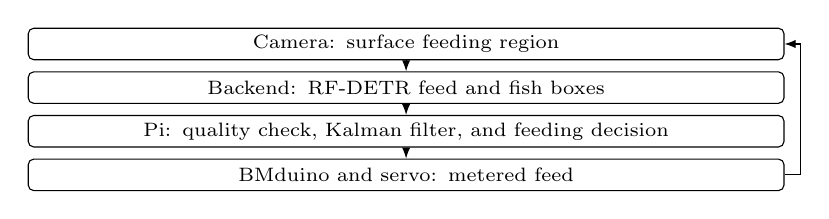
\begin{tikzpicture}[font=\scriptsize,box/.style={draw,rounded corners=2pt,align=center,text width=.78\columnwidth,minimum height=4mm,inner sep=2pt},arr/.style={-{Latex[length=1.4mm]},thin},node distance=1.4mm]
\node[box] (cam) {Camera: surface feeding region};
\node[box,below=of cam] (det) {Backend: RF-DETR feed and fish boxes};
\node[box,below=of det] (pi) {Pi: quality check, Kalman filter, and feeding decision};
\node[box,below=of pi] (act) {BMduino and servo: metered feed};
\draw[arr] (cam)--(det); \draw[arr] (det)--(pi); \draw[arr] (pi)--(act);
\draw[arr] (act.east)--++(2mm,0)|-(cam.east);
\end{tikzpicture}
\caption{Closed-loop architecture. The Pi controls feeding; the backend performs detection.}
\label{fig:system}
\end{figure}

\begin{figure}[H]
\centering
\includegraphics[width=.50\columnwidth]{feeding_device.jpg}
\caption{Prototype feeder with BMduino, Raspberry Pi, and servo-driven outlet.}
\label{fig:device}
\end{figure}

\subsection{Visible-Feed Measurement}
For frame $t$, let $B_i$, $w_i$, $h_i$, $c_i$, and $y_i$ be the box, its width, height, confidence, and class of detection $i$. Within a fixed region of interest $\Omega$, the visible-feed proxy is
\begin{equation}
\begin{aligned}
A_t={}&\sum_{i=1}^{N(t)}w_i h_i\mathbb{I}(y_i=\mathrm{feed})\\
&\cdot\mathbb{I}(c_i\geq\tau)\mathbb{I}(B_i\cap\Omega\neq\varnothing).
\end{aligned}
\label{eq:area}
\end{equation}
$A_t$ is neither pellet mass nor an exact pellet count; overlapping boxes and boxes crossing the region boundary can bias it. The supplied example overlay (Fig.~\ref{fig:detection}) illustrates why only feed-class boxes enter $A_t$. It is not an accuracy result.

\begin{figure}[H]
\centering
\includegraphics[width=.50\columnwidth]{detection.png}
\caption{Example detection overlay. Only feed-class boxes within the observation region contribute to $A_t$.}
\label{fig:detection}
\end{figure}

\subsection{Filtering and Decision Rule}
Glare, occlusion, ripples, and missed detections make $A_t$ noisy. A quality gate checks aggregate feed confidence, occlusion, glare, and the filter innovation. With $z_t=A_t$, a causal one-dimensional random-walk Kalman filter~\cite{kalman1960} uses
\begin{equation}
x_t=x_{t-1}+q_t,\qquad q_t\sim\mathcal{N}(0,Q),
\label{eq:process}
\end{equation}
\begin{equation}
z_t=x_t+v_t,\qquad v_t\sim\mathcal{N}(0,R),
\label{eq:measurement}
\end{equation}
\begin{equation}
\begin{aligned}
\hat x_{t\mid t-1}&=\hat x_{t-1\mid t-1},\\
P_{t\mid t-1}&=P_{t-1\mid t-1}+Q,
\end{aligned}
\label{eq:prediction}
\end{equation}
\begin{equation}
K_t=\frac{P_{t\mid t-1}}{P_{t\mid t-1}+R},
\label{eq:gain}
\end{equation}
\begin{equation}
\hat x_{t\mid t}=\hat x_{t\mid t-1}+K_t(z_t-\hat x_{t\mid t-1}),
\label{eq:update}
\end{equation}
\begin{equation}
\begin{aligned}
P_{t\mid t}&=(1-K_t)P_{t\mid t-1},\\
\hat A_t&=\max(0,\hat x_{t\mid t}).
\end{aligned}
\label{eq:posterior}
\end{equation}
Here $Q$ and $R$ are process- and measurement-noise variances. Invalid frames use prediction only and cannot trigger an increase in feed. $Q$, $R$, and quality limits will be set with annotated calibration data.

After a calibrated portion $g(u_k)$ is dispensed, the controller waits for falling feed to settle, then observes for $L$ scheduled frames. Frames that fail the quality gate receive prediction only. If too few frames are valid, the controller suspends further feeding. Otherwise, it compares the first and last filtered measurements using
\begin{equation}
\rho_t=\frac{\hat A_{t-L}-\hat A_t}{\max(\hat A_{t-L},\varepsilon)},\qquad L\in\mathbb{N}^{+}.
\label{eq:rho}
\end{equation}
A larger positive $\rho_t$ indicates faster disappearance of visible feed. If $\rho_t\geq\theta_H$, the next portion may increase; if $\theta_L\leq\rho_t<\theta_H$, it stays at baseline; otherwise it decreases or pauses (Fig.~\ref{fig:demand}). Hysteresis, minimum state duration, and portion limits prevent rapid switching and overfeeding. No measurement is used while the motor runs or feed falls.

\begin{figure}[H]
\centering
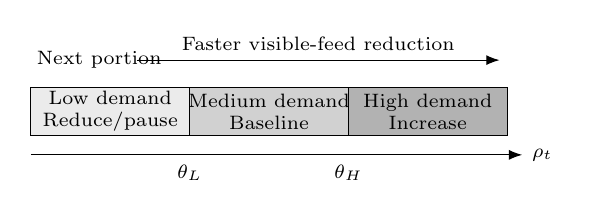
\begin{tikzpicture}[x=.96cm,y=.64cm,font=\scriptsize,>=Latex]
\node[anchor=west] at (.55,2.2) {Next portion};
\draw[->] (2.0,2.2)--(6.8,2.2) node[midway,above] {Faster visible-feed reduction};
\filldraw[fill=black!8,draw=black] (.6,.7) rectangle (2.7,1.65);
\filldraw[fill=black!18,draw=black] (2.7,.7) rectangle (4.8,1.65);
\filldraw[fill=black!30,draw=black] (4.8,.7) rectangle (6.9,1.65);
\node[align=center] at (1.65,1.18) {Low demand\\Reduce/pause};
\node[align=center] at (3.75,1.18) {Medium demand\\Baseline};
\node[align=center] at (5.85,1.18) {High demand\\Increase};
\draw[->] (.6,.32)--(7.1,.32) node[right] {$\rho_t$};
\node[below] at (2.7,.32) {$\theta_L$};
\node[below] at (4.8,.32) {$\theta_H$};
\end{tikzpicture}
\caption{Relative visible-feed reduction and demand levels. The dimensionless $\rho_t$ is measured per observation window.}
\label{fig:demand}
\end{figure}

\section{System Validation and Discussion}
Following the development of the proposed framework and prototype, validation is structured from perception to deployment (Table~\ref{tab:validation}).

Feed and fish boxes are annotated on images from the intended camera viewpoint. Detection performance is evaluated using precision, recall, F1, mAP@0.5, and mAP@0.5:0.95. Errors are also examined by pellet size, surface glare, and fish occlusion, as feeding decisions depend on reliable feed detection.

\begin{table}[H]
\caption{\textsc{System Validation Framework and Evaluation Measures}}
\label{tab:validation}
\centering
\small
\renewcommand{\arraystretch}{1.0}
\begin{tabularx}{\columnwidth}{@{}p{.19\columnwidth}>{\raggedright\arraybackslash}X@{}}
\hline
\textbf{Level} & \textbf{Measure and comparison} \\ \hline
Detection & Precision, recall, F1, mAP@0.5, mAP@0.5:0.95 for feed boxes \\
Signal & Area error, temporal variance, response delay; raw versus EMA versus Kalman \\
Control & Feed mass, visible uneaten-feed duration, final biomass, mortality, water quality, FCR \\
Deployment & Inference and network latency, acquisition-to-actuation delay, frame rate, power \\ \hline
\end{tabularx}
\end{table}

At the signal level, manually marked feed masks or visible-pellet counts provide reference measurements. Raw box area, exponential moving average, and causal Kalman estimates are compared for error, variance, and response delay. Offline smoothing serves only as an analysis reference. Dispensing is calibrated by weighing repeated servo cycles to establish the feed mass $g(u_k)$ for each command $u_k$.

Feeding evaluation compares the proposed adaptive strategy with timer-based feeding using tanks with matched initial biomass. Measures include total dispensed feed, visible uneaten-feed duration, final biomass, mortality, water quality, and FCR. Group differences are assessed using effect sizes and confidence intervals. Deployment evaluation includes inference time, network round-trip time, acquisition-to-actuation delay, frame rate, and power consumption.

The visible-feed proxy does not capture sinking feed and may be affected by camera viewpoint, glare, and fish occlusion. Dispensing mass, camera geometry, and safety limits therefore require calibration under controlled tank conditions. The measure in Eq.~\eqref{eq:rho} represents visible-feed disappearance and is interpreted as a physical response proxy rather than a direct measurement of actual consumption.

\section{Conclusion}
This study presents a Physical AI framework for adaptive aquaculture feeding based on visual feed dynamics. The framework integrates RF-DETR-based perception, causal temporal estimation, and embedded actuation to incorporate observed physical responses into subsequent feeding decisions. This approach provides a foundation for responsive and resource-aware feeding, with potential benefits for reducing unnecessary feed use and supporting environmentally sustainable aquaculture.

\begin{thebibliography}{6}
\bibitem{foster1995} M. Foster, R. Petrell, M. R. Ito, and R. Ward, ``Detection and counting of uneaten food pellets in a sea cage using image analysis,'' \emph{Aquacultural Engineering}, vol. 14, no. 3, pp. 251--269, 1995.
\bibitem{liu2014} Z. Liu, X. Li, L. Fan, H. Lu, L. Liu, and Y. Liu, ``Measuring feeding activity of fish in RAS using computer vision,'' \emph{Aquacultural Engineering}, vol. 60, pp. 20--27, 2014.
\bibitem{zhou2018} C. Zhou \emph{et al.}, ``Near infrared computer vision and neuro-fuzzy model-based feeding decision system for fish in aquaculture,'' \emph{Computers and Electronics in Agriculture}, vol. 146, pp. 114--124, 2018.
\bibitem{robinson2026} I. Robinson, P. Robicheaux, M. Popov, D. Ramanan, and N. Peri, ``RF-DETR: Neural Architecture Search for Real-Time Detection Transformers,'' in \emph{Proc. ICLR}, 2026.
\bibitem{kalman1960} R. E. Kalman, ``A new approach to linear filtering and prediction problems,'' \emph{Journal of Basic Engineering}, vol. 82, no. 1, pp. 35--45, 1960.
\end{thebibliography}
\end{document}
